\documentclass[a4paper,11pt,dvipdfmx]{jsarticle}

\usepackage{bm}
\usepackage[dvipdfmx]{graphicx}
\usepackage[dvipdfmx]{color}
\usepackage{ascmac}
\usepackage{siunitx}
\usepackage{otf}
\pagestyle{plain}
\usepackage{float}
\usepackage[dvipdfmx]{hyperref}
\usepackage{pxjahyper}
\usepackage{here}
\usepackage{titlesec}
\usepackage{amsmath,amssymb} %北野加筆
\renewcommand{\bibname}{参考文献} %北野加筆
\titleformat*{\section}{\LARGE\bfseries}
\titleformat*{\subsection}{\normalsize\bfseries}
\usepackage[subrefformat=parens]{subcaption}
\usepackage{url}
\usepackage{comment}
\usepackage{docmute}
\setcounter{page}{0}
\usepackage[table,xcdraw]{xcolor}
\hypersetup{% hyperrefオプションリスト
setpagesize=false,
 bookmarksnumbered=true,%
 bookmarksopen=true,%
 colorlinks=true,%
 linkcolor=blue,
 citecolor=blue,
}


\begin{document}

\newpage

\subsection{微分散乱断面積}
ここでは実験で得られたデータから微分散乱断面積を求めるための理論式を導出する。また解析を行う際に行った補正式についても触れる。

\subsubsection{微分散乱断面積の算出}
ここでは物理量を次のように定義する。
\begin{table}[h]
\small
\it
\centering
\begin{tabular}{ll} 

  $d\Omega$:微小立体角 {\rm [sr]} & n:ターゲット原子核の面密度 {\rm [/cm$^2$]}\\
  N:d$\Omega$に散乱された粒子数 & $N_{all}$:全粒子数 \\ 
  d:ターゲットの密度 {\rm[g/cm$^3$]} & t:ターゲットの厚み {\rm[cm]} \\ 
  N$_A$:アボガドロ数 {\rm[/mol]} & r:二次電子抑制管の穴の半径 {\rm[cm]} \\ 
  l:散乱点から検出器までの距離 {\rm[cm]} & I:陽子ビームの電流値 {\rm[A]} \\ 
  T:計測時間 {\rm[s]} & e:素電荷 {\rm[C]}\\
  A:ターゲット原子の質量数 {\rm[g/mol]}
  \label{def1}
\end{tabular}
\end{table}

\noindent
    面密度{\it n}のターゲットに陽子ビームを照射し、{\it d$\Omega$}の範囲で観測することを考える。単位立体角あたりに陽子が散乱される確率は微分散乱断面積と面密度の積で与えられるから、

\begin{equation}
    \centering
    \frac{d\sigma}{d\Omega} \times n \times d\Omega = \frac{N}{N_{all}} 
\end{equation}
と表される。またそれぞれの値は
\begin{eqnarray}
    \centering
    &n = \frac{d \times t \times N_A}{A}&\\
    &d\Omega = \frac{\pi{r^2}}{l^2}&\\
    &N_{all} = \frac{IT}{e}&
\end{eqnarray}

の3式で求められる。これらから、微小立体角$d\Omega$における微分散乱断面積$\frac{d\sigma}{d\Omega}$は\eqref{eq:expcs}式で表すことができる。

\begin{equation}
    \frac{d\sigma}{d\Omega} = \frac{l^2 \times N \times e \times A}{\pi{r^2} \times I \times T \times d \times t \times N_A}
    \label{eq:expcs}
\end{equation}


\newpage
\subsubsection{各パラメーターの決定}
\eqref{eq:expcs}式をもとに、各角度における微分散乱断面積を求める際のパラメーターを決定する。ここではパラメーター決定の方法とそれぞれの誤差について説明する。

\begin{description}
   \item[● 散乱粒子数 ${\it N}$]\mbox{}\\
   エネルギースペクトルの対応するピークを積分することで求めた。スペクトル上にガウスピークが見られる場合はMean値から$\pm3\sigma$の範囲を積分した。3$\sigma$の範囲で積分することで、理論的に99.7\%の粒子数をカウントすることができる。また図\ref{PE140}のような分布に関しては、複数のガウシアンでフィッティングを行うことで$3\sigma$の値を決定し、積分を行った。 
   
   \vspace*{5mm}
   
    \begin{figure}[H]
     \begin{tabular}{cc}
       \begin{minipage}[t]{0.45\hsize}
        \centering
        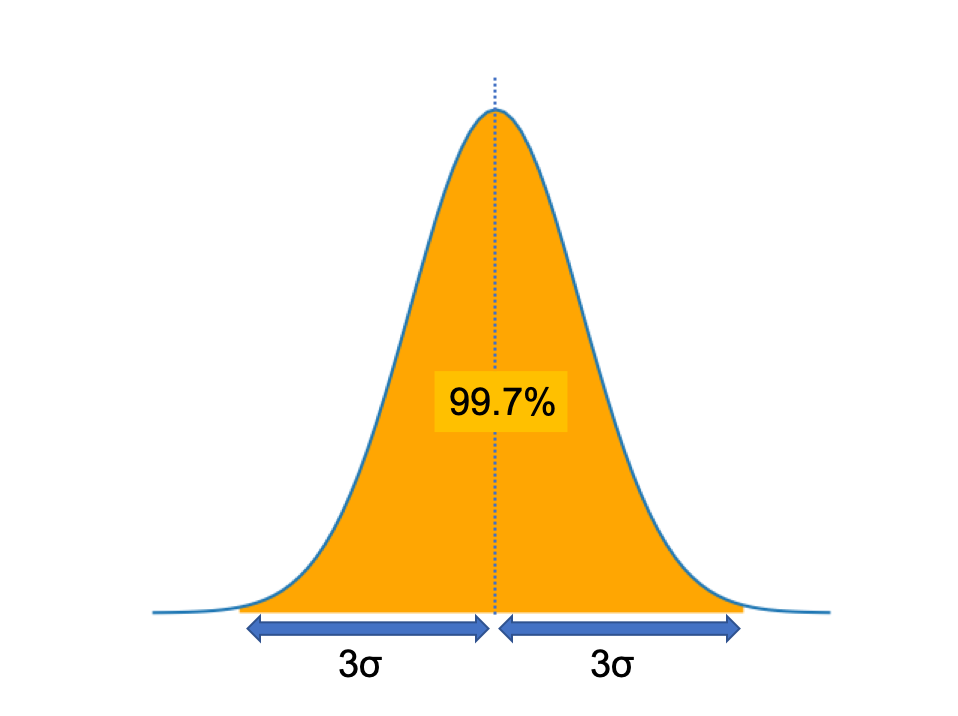
\includegraphics[width=60mm,height=42mm]{picture/CS/3sigma.png}
        \caption{ガウシアンにおける3$\sigma$}
        \label{3sigma}
       \end{minipage} &
       \begin{minipage}[t]{0.45\hsize}
        \centering
        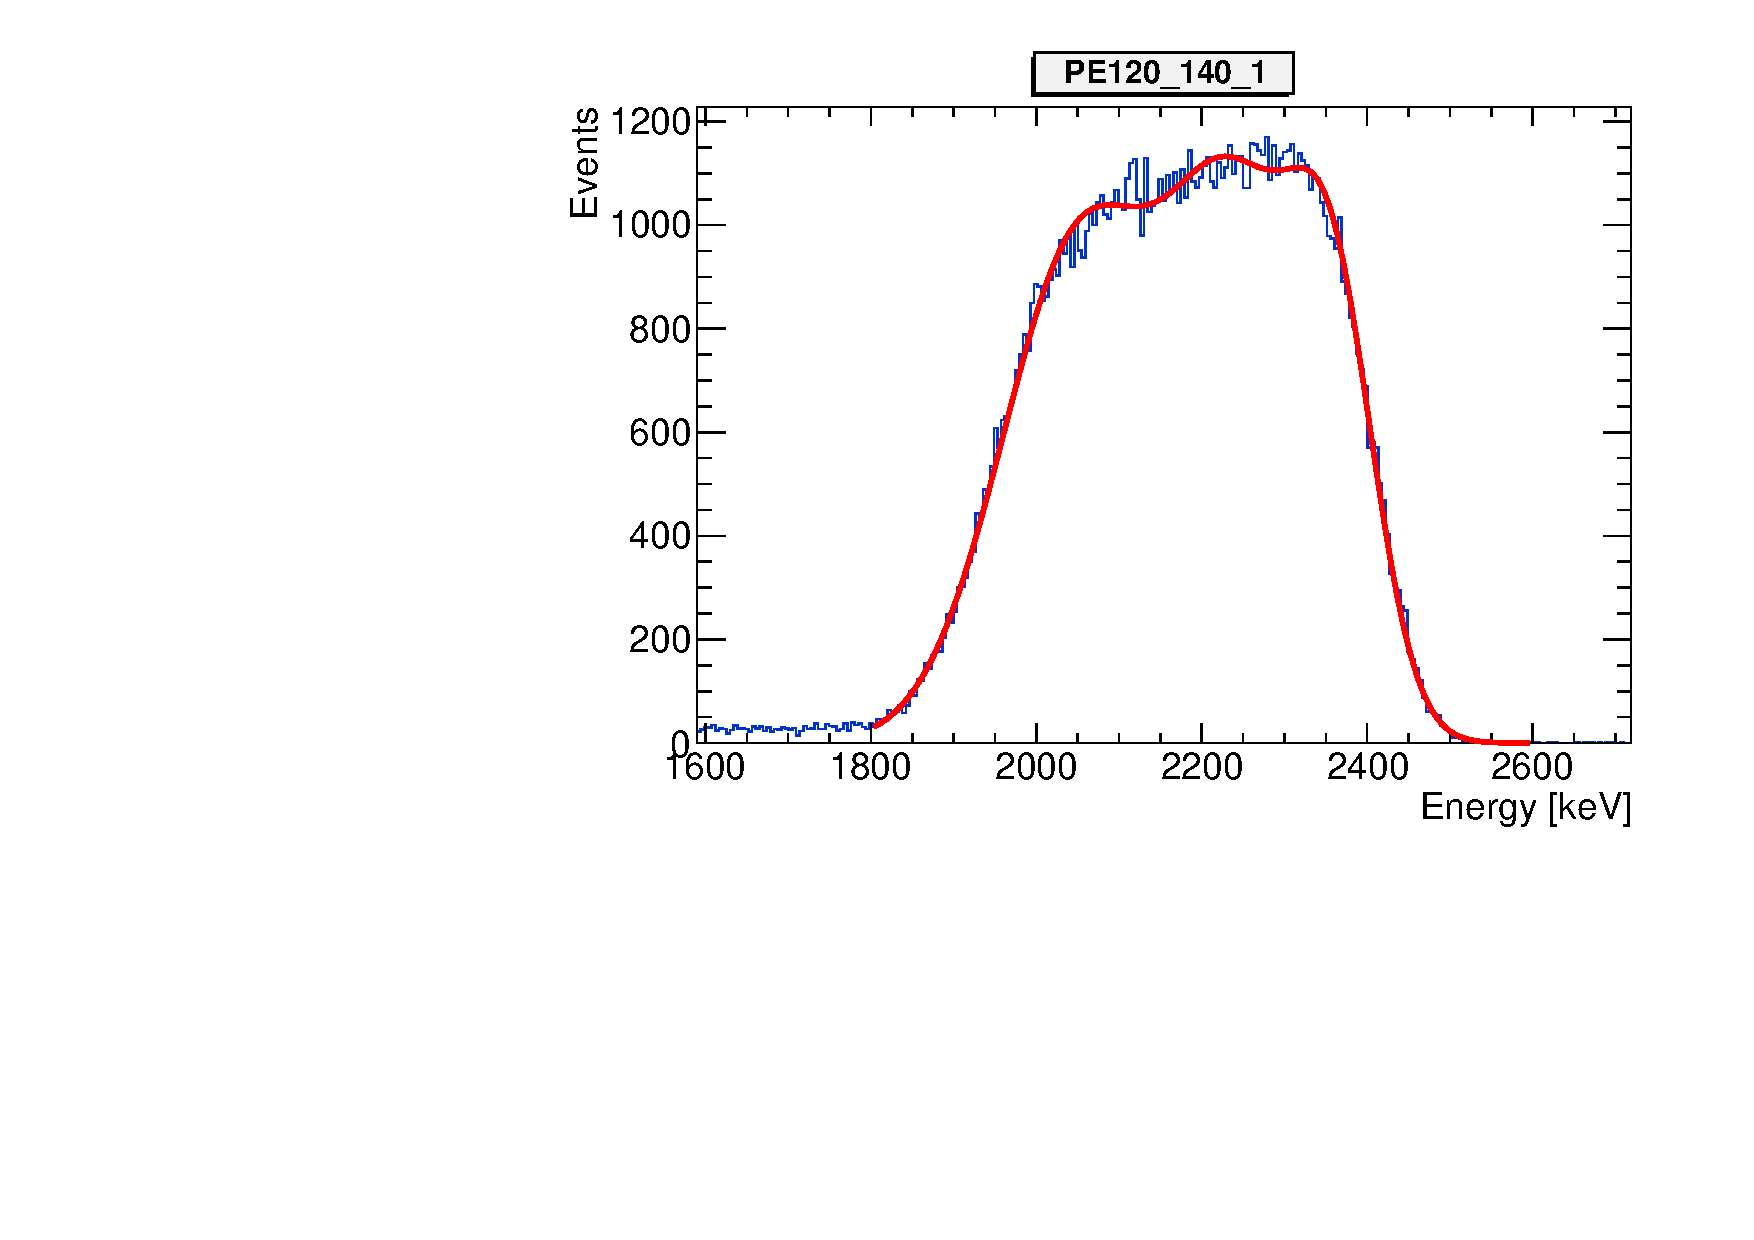
\includegraphics[width=60mm,height=42mm]{picture/CS/PE120_140_1.pdf}
        \caption{複数のガウシアンによるfitting}
        \label{triplegauss}
       \end{minipage}
     \end{tabular}
   \end{figure}
  また誤差${\it \sigma_N}$ = $\sqrt{N}$ とした。\\
   
  \item[● 電流値 ${\it I}$]\mbox{}\\
   ビームの強度を表す電流値{\it I}は、ビームストッパーと導通している二次電子抑制管に流れる電流値を測定することで決定した。計測は5秒ごとに行い、ビームタイムの中での平均値を実験値とした。計測にはT\&D社のデータロガーを用いた。誤差${\it \sigma_I}$には平均値を最確値とした標準誤差を使用した。\\
  
  \item[● 計測時間{\it T}]\mbox{}\\
   MCAでの計測におけるLive timeを${\it T}$とし、本研究では${\it T}$ = 100 [s]で計測を行った。\\
\end{description}

\newpage
\subsubsection{誤差の算出}
$n$個の変数からなる関数$f(x_1,x_2,\cdots,x_n)$を考える。変数${ x_i}$の誤差$\sigma_{x_i}$が互いに独立であるなら、その関数の誤差$\sigma_f$は\eqref{eq:err1}式のように表される。

\begin{equation}
\centering
\sigma_f = \sqrt{\sum_{i=1}^{n} \left(\frac{\partial f}{\partial x_i} {\sigma_{x_i}}\right)^2}
\label{eq:err1}
\end{equation}

\noindent
本研究では\eqref{eq:expcs}式における誤差を含むパラメーターを $N$、$I$、$d$、$t$と設定した。$g = \frac{d\sigma}{d\Omega}$とし、
それぞれの誤差を伝播させて\eqref{eq:err2}式で算出を行った。

\begin{equation}
\centering
\sigma_g = \sqrt{ \left(\frac{\partial g}{\partial N} {\sigma_N }\right)^2 + \left(\frac{\partial g}{\partial I} {\sigma_I }\right)^2 + \left(\frac{\partial g}{\partial d} {\sigma_d }\right)^2 + \left(\frac{\partial g}{\partial t} {\sigma_t }\right)^2}
\label{eq:err2}
\end{equation}


\subsubsection{角度の補正}
Rutherfordの散乱公式\eqref{eq:Rutherford}における角度$\theta$は重心系である。本実験での計測は実験室系の角度を用いていたため、補正を行う必要がある。変換公式は以下のように与えられる。
\begin{equation}
    \tan \theta_{lab} = \frac{\sin \theta_{cm}}{M_1/M_2 + \cos {\theta_{cm}}}
\end{equation}

\begin{table}[h]
\small
\centering
\begin{tabular}{ll} 
    $\theta_{lab}$:散乱角度(実験室系)[$^\circ$] & $\theta_{cm}$:散乱角度(重心系)[$^\circ$] \\
    $M_1$:入射粒子の質量数 & $M_2$:標的原子の質量数
    \label{def2}
\end{tabular}
\end{table}

\noindent
入射粒子は陽子(水素原子核)であるため、$M_1 = 1$である。標的が金のとき$1/M_2$は十分に小さいため$\theta_{lab} \simeq \theta_{cm}$となるが、炭素原子核や水素原子核がターゲットのときには大きなずれが生じるので補正を行った。水素原子核がターゲットのときは、$\theta_{cm} = 2      \theta_{lab}$で表される。

\subsubsection{散乱公式の補正}\label{kakuhosei}
\eqref{eq:Rutherford}式は入射粒子の質量がターゲット原子核の質量より十分小さいことを条件とするものである。炭素原子核を標的とするとき、その質量比は無視できないので換算質量への補正を行う必要がある。換算質量を$\mu$とすると、
\begin{equation}
\frac{1}{\mu} = \frac{1}{M_1} + \frac{1}{M_2}
\end{equation}
で表される。

\newpage
\subsubsection{核力による散乱の補正}
\ref{NF}節において、核力による散乱における微分散乱断面積を導出した。しかしこれは古典的な導出であるので、ここでは入射粒子を平面波として扱って導出する。物理量を以下のように定義する。
\begin{table}[h]
\small
\it
\centering
\begin{tabular}{ll} 
    R:ターゲット原子核の半径 & $\lambda$:陽子の{\rm de Broglie}波長\\
    h:プランク定数 & k:波数\\
    l:軌道角運動量 & $\delta$:位相差\\
    $\mu$:換算質量 & $\sigma$:全散乱断面積\\
    $m_{p}$:陽子の質量 & p:{\rm3 MeV}の陽子の運動量\\
    $f(\theta)$:散乱角$\theta$における散乱振幅
    
\label{def3}
\end{tabular}
\end{table}

運動する物体は波の性質を持っており、そのde Brogrie波長は(\ref{dB})式のように表される。今回用いたのは3 MeVの陽子であるので、その波長は$\lambda \simeq 16.53$ fmである。\\
\begin{equation}
    \lambda = \frac{h}{p} = \frac{h}{m_{p}v}
    \label{dB}
\end{equation}\\
ここでは入射平面波と反射球面波を部分波展開することで、散乱球面波の位相の変化から散乱断面積を導出する。
%入射平面波と反射平面波の振幅の絶対値は等しくなるはずなので、
%\begin{equation}
 %   |1 + 2ikf_l(\theta)| = 1
%\end{equation}
散乱ポテンシャルV(r)が球対称な場合、散乱振幅はルジャンドル多項式を用いて級数展開することができ、\\
\begin{equation}
    f(\theta) = \sum_{l=0}^{\infty} (2l+1) \: f_l \: P_l (cos\theta) 
\end{equation}\\
のように書ける。ここで$f_l$は部分波振幅である。散乱の前後で粒子の湧き出しや吸い込みはないので、入射波と反射波の振幅は等しくなければならない。$\delta_l$を剛体球がない場合の散乱波とある場合の位相の差とすると、\\
\begin{equation}
    e^{2i\delta_l} = 1 + 2ikf_l
    \label{sinpuku}
\end{equation}\\
と定義される。波動関数の動径方向に関するSchr\"{o}dinger方程式(\ref{sch})を解き、剛体球がない場合の位相と比較を行うと、部分波振幅$f_l$は(\ref{sinpuku})式の結果より(\ref{bubun})式のように与えられる。\\
\begin{equation}\\
    \left[-\frac{\hbar^2}{2\mu}\left\{\frac{d}{dr}-\frac{l(l+1)}{r^2}\right\} + V(r)\right]\psi_l(r) = \frac{\hbar^2k^2}{2\mu}\psi_l(r)
    \label{sch}
\end{equation}
\begin{equation}
    f_l = \frac{e^{i\delta_l}\sin \delta_l}{k}
    \label{bubun}
\end{equation}
以上より、全散乱断面積$\sigma$は(\ref{zendan})式のように表される。
\begin{eqnarray}
    \sigma &=& \int |f(\theta)|^2 d\Omega\\
    &=& \frac{4\pi}{k^2}\sum_{l}(2l+1)\sin^2 \delta_l
    \label{zendan}
\end{eqnarray}

\noindent
核力による散乱を剛体球による散乱と仮定すると、その散乱ポテンシャル$V(r)$は剛体球の中心を原点とした座標rを用いて\\
\begin{equation}
    V(r) = \begin{cases}
    \infty & (r < R)\\
    0 & (r > R)
    \end{cases}
\end{equation}\\
のように表される。剛体球の中には入射平面波は侵入できないので、$r=R$で$\psi=0$となる。したがって位相差$\delta_l$は、
\begin{eqnarray}
    kR + 2\delta_l &=& -( kR - \pi l)\\
   \delta_l &=& \frac{\pi l}{2} - kR 
\end{eqnarray}
のように表される。$k=\frac{2\pi}{\lambda}$より、入射平面波の波長$\lambda$とポテンシャルの及ぶ範囲$R$の相対的な関係により位相差$\delta_l$が変化することがわかる。ここで、$\lambda$が$R$に対して十分に大きい場合を考えると、$l=0$の成分(S波)のみを考えればよく、$\delta_l=-kR$となる。したがって全断面積$\sigma$は(\ref{sigma})式で表される。またS波は等方的に散乱されるため、核力による微分散乱断面積は、(\ref{kakubibun})式で与えられる。\\
\begin{equation}
    \sigma = \frac{4\pi}{k^2}\sin^2 {\delta_l}
    \label{sigma}
\end{equation}
\begin{equation}
   \frac{d\sigma}{d\Omega} = \left(\frac{\sin \delta_l}{k}\right)^2
   \label{kakubibun}
\end{equation}\\
ここで$\delta_l \ll 1$とすると、$\sin \delta_l \simeq \delta_l$と近似できるので\eqref{eq:NFcs}式のように表され、幾何学的に求めた古典的な散乱断面積(\ref{eq:nfcr2})の4倍となることが分かる。\\
\begin{equation}
    \frac{d\sigma}{d\Omega} \simeq R^2
    \label{eq:NFcs}
\end{equation}

\end{document}